\section{Implementation Details}
\label{sec:implementation}



\subsection{Model and Training Configuration}
\label{sec:model_configuration}
\label{sec:training_configuration}
\label{sec:train_infer_consistency}

\ourmodel supports both dense and mixture-of-experts (MoE) architectures across Qwen3-VL and Qwen3.5 families. The trained models share the same autoregressive keyboard-mouse action interface without an additional output head. We first analyze CPT scaling across 120 controlled Qwen3.5 Dense configurations, referred to as \textbf{GameScaling}. Guided by these findings, we train \ourmodel from Qwen3-VL-8B with additional HSR gameplay data.

Training follows three stages while preserving the model architecture and action representation. CPT learns transferable control with key remapping and repeat-aware loss decay. SFT introduces multi-level task supervision, sparse reasoning, and cross-context memory. TA-GRPO then improves long-horizon behavior through online interaction, using environment-verifiable rewards and temporal credit assignment. Gameplay trajectories are sampled at 5~Hz, with six action blocks per step providing approximately 30~Hz control and a local visual history of 20 frames.

We extend Verl~\cite{sheng2024hybridflow} into a unified training and evaluation framework, using \textbf{Streaming-vLLM} for interactive evaluation and online RL rollouts. A sharded inference service pool backed by \textbf{64 NVIDIA H200 GPUs} serves 32 parallel game environments. Each RL iteration collects 128 rollouts in groups of 8, with environment-verifiable rewards and no learned process reward model. Updated policy weights are synchronized across the service pool before the next rollout collection, keeping policy versions aligned throughout online training. Streaming-vLLM also supports dense and MoE backbones on NVIDIA A800 and H200 GPUs. Further configuration details are provided in Table~\ref{tab:training_recipe} and Appendix~\ref{app:unified_training_inference}.

\begin{figure*}[!htbp]
    \centering
    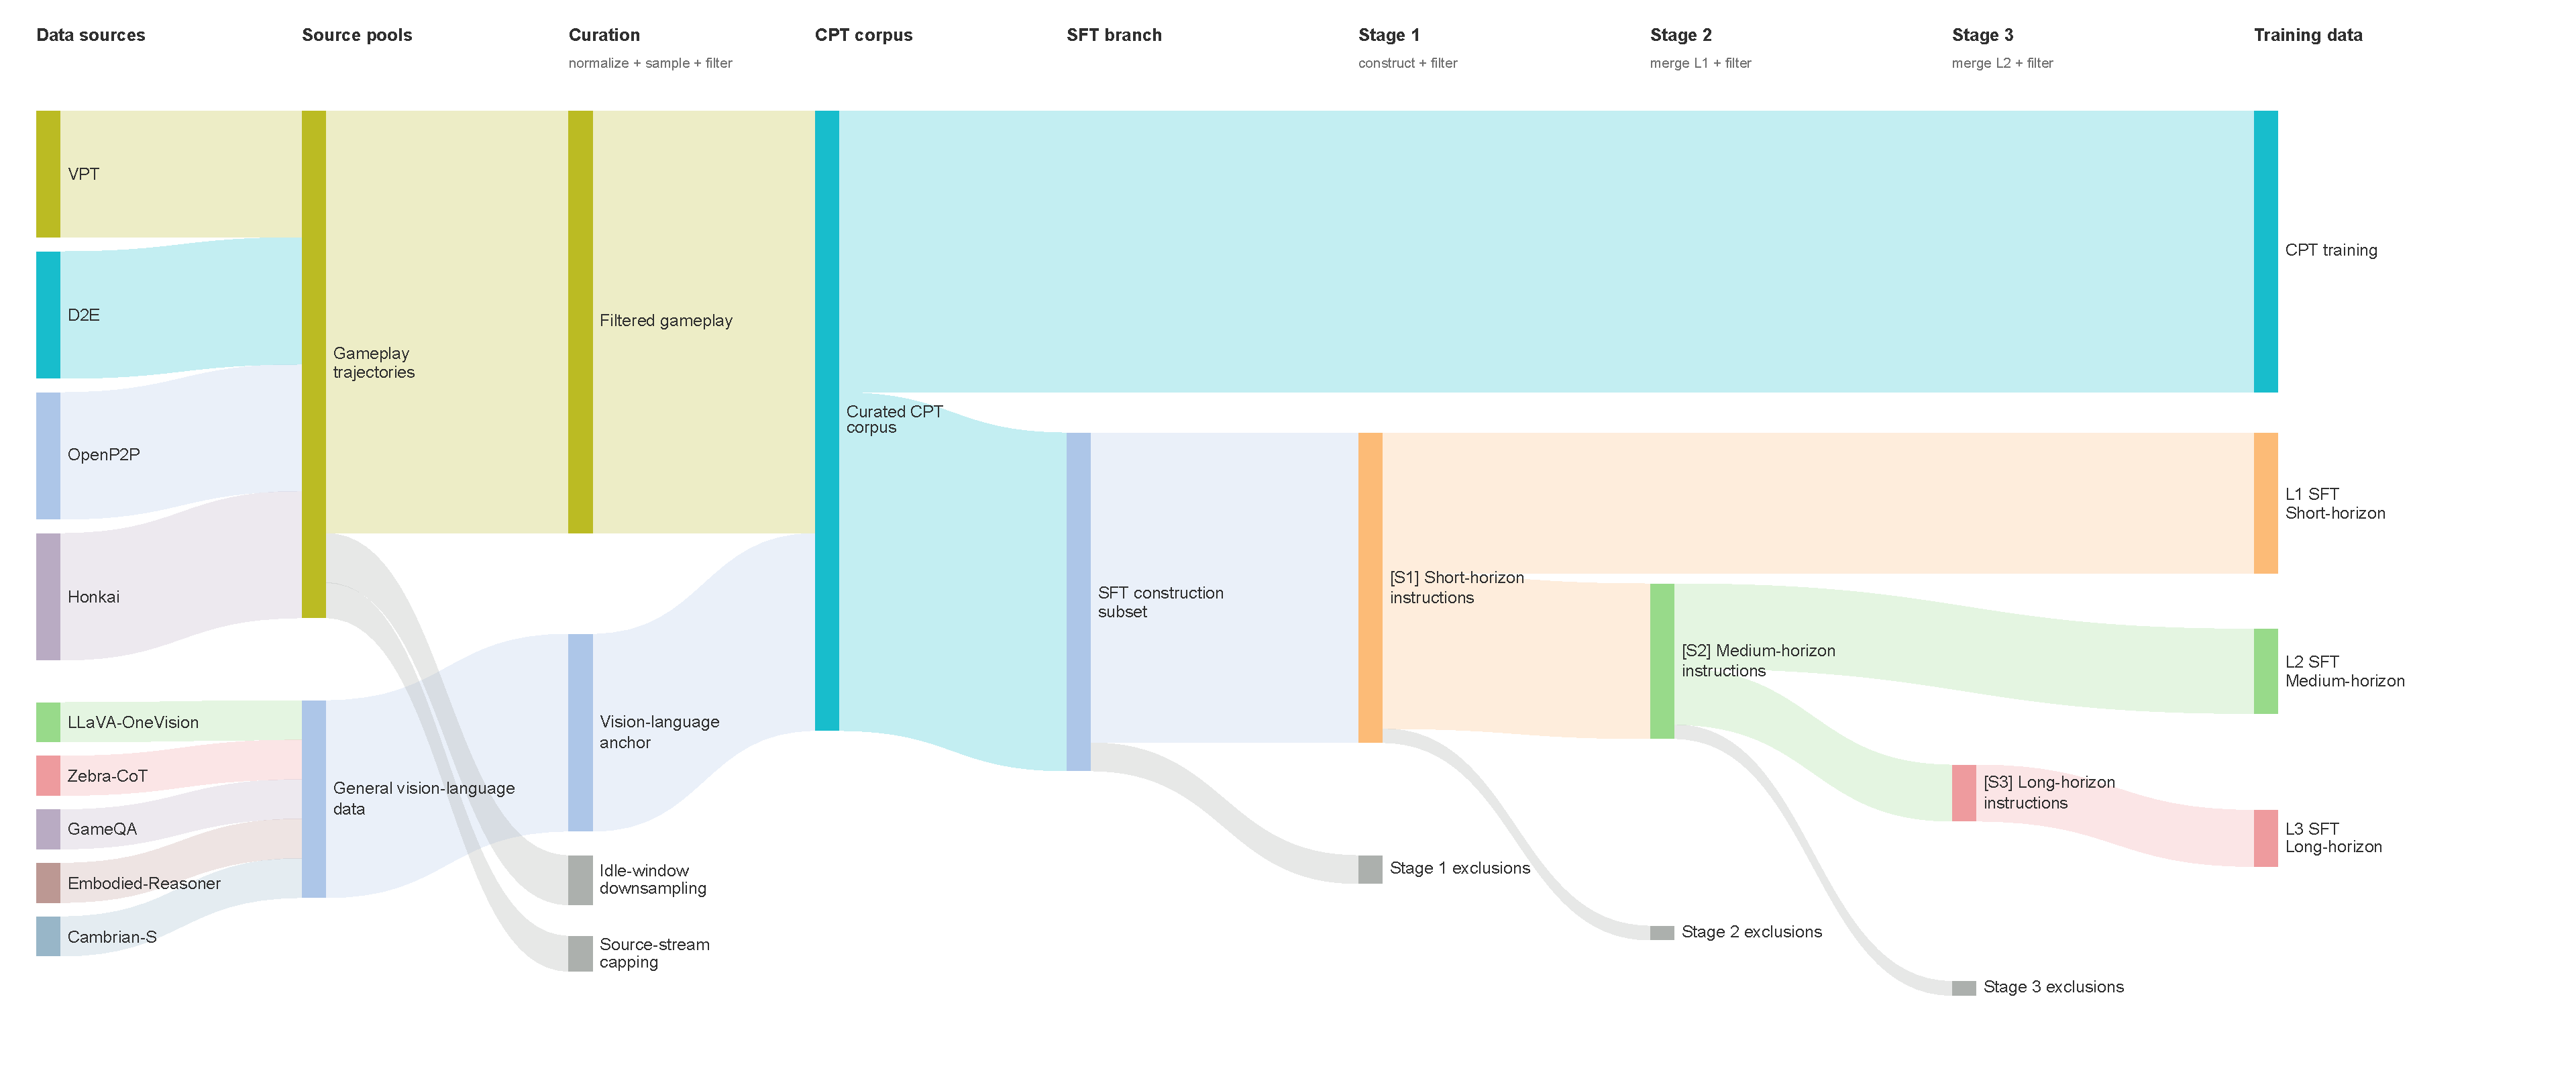
\includegraphics[width=0.88\linewidth]{figs/cpt_sft_sankey.pdf}
    \caption{
    \textbf{Multi-stage data curation for training.}
    Gameplay trajectories and general vision-language data are cleaned, sampled, and filtered to construct the CPT corpus.
    Trajectories with aligned action annotations are further used to construct SFT examples at three levels: short-horizon operations, medium-horizon subgoals, and long-horizon tasks.
    For RL, online policy interaction provides trajectories and environment-verifiable outcomes.
    }
    \label{fig:training_data_flow}
\end{figure*}


The controlled scaling study spans 120 CPT configurations and approximately 45K H200 GPU-hours. Shorter training budgets are derived from shared Warmup-Stable-Decay trajectories with separate final decay phases. For the subsequent \ourmodel training stages, CPT uses a distributed H200 cluster, SFT uses a distributed A800 cluster, and online RL uses Megatron/MCore with BF16 optimization. Real-time rollouts run in parallel game environments served by a sharded Streaming-vLLM pool backed by 64 H200 GPUs. The pool receives synchronized policy checkpoints between rollout iterations, enabling consistent interaction data collection as training progresses. More details of training configurations and stage-specific settings are summarized in Table~\ref{tab:training_recipe}.

\subsection{Data Composition and Sampling}
\label{sec:data_composition}

Our training data combines cross-game interaction trajectories, general multimodal data, multi-level task supervision, and online policy experience. Figure ~\ref{fig:training_data_flow} summarizes how these sources are filtered and routed into the CPT, SFT, and RL stages, while Table~\ref{tab:data_summary} reports their corresponding usage and scale.



In the CPT stage, we perform controlled scaling experiments (i.e., GameScaling) using a mixture of VPT~\cite{baker2022vpt}, D2E~\cite{choi2026d2e}, and OpenP2P~\cite{yue2026openp2p} gameplay data while holding the token ratio at 85\% gameplay and 15\% general vision-language data (Appendix~\ref{app:cpt_diversity}). General multimodal data sources include LLaVA-OneVision~\cite{llava-o}, Zebra-CoT~\cite{li2026zebracot}, GameQA~\cite{tong2026gamerl}, Embodied-Reasoner~\cite{zhang2025embodiedreasoner}, and Cambrian-S~\cite{yang2025cambrians}. \ourmodel's CPT stage retains this data mixture ratio and adds additional HSR gameplay trajectories.

In the SFT stage, we annotate approximately 1K hours of curated HSR gameplay trajectories. As described in Sec.~\ref{sec:multi-level_supervision}, operation-level examples train local control and sparse reasoning. Subgoal-level examples add intermediate objectives and longer memory, while task-level examples cover complete long-horizon tasks. Examples at different annotation levels may come from the same trajectory and we count their derived samples and supervision tokens separately. 

To improve coverage across gameplay scenarios, we downsample overrepresented streams and excessively idle intervals while preserving meaningful movement, held controls, and waiting periods. In the HSR portion of the CPT corpus, filtering retains approximately 149K aligned clips, corresponding to around 332 hours of gameplay. Data splits are assigned at the recording or complete-task level before creating overlapping windows or multi-level examples, so derived samples from a source remain in the same split.

\begin{table*}[t]
\centering
\small
\caption{
\textbf{Overview of training data used for building \ourmodel.}
The table summarizes the major data sources, their role in each training stage, and the corresponding data scale.
}
\label{tab:data_summary}

\resizebox{0.98\linewidth}{!}{%
\begin{tabular}{lllcc}
\toprule

\textbf{Stage}
& \textbf{Data}
& \textbf{Supervision / Usage}
& \textbf{Size}
& \textbf{Sampling} \\

\midrule

\multirow{4}{*}{CPT}
& VPT, D2E, OpenP2P
& \multirow{2}{*}{Cross-game generalization}
& \multirow{2}{*}{ \ensuremath{\sim}2.4K hours}
&  \multirow{2}{*}{85\%} \\
& Honkai: Star Rail (HSR) 
& & & \\
\cmidrule{2-5}

& LLaVA-OneVision, Zebra-CoT, GameQA
  
& Vision–language 
& \multirow{2}{*}{\ensuremath{\sim}6.3B tokens}
& \multirow{2}{*}{15\%} \\

& Embodied-Reasoner, Cambrian-S
& Embodied and egocentric 
& & \\

\midrule

\multirow{3}{*}{SFT}
& Operation-Level HSR
& Local operations
& \ensuremath{\sim}261K samples
& 37.0\% \\

\cmidrule{2-5}

& Subgoal-Level HSR
& Intermediate subgoals
& \ensuremath{\sim}211K samples
& 29.8\% \\

\cmidrule{2-5}

& Task-Level HSR
& Long-horizon task
& \ensuremath{\sim}234K samples
& 33.1\% \\


\midrule

RL
& Verified Online Trajectories
& Policy optimization
& \ensuremath{\sim}14.6K rollouts
& -- \\

\bottomrule
\end{tabular}
}
\vspace{-4pt}
\end{table*}



\subsection{Automated RL Environment}
\label{sec:rl_environment}

\textbf{A shared infrastructure for learning, evaluation, and testing.}
Many existing game-RL benchmarks run as lightweight, self-contained simulators that can be reset cheaply and queried directly for rewards. Modern commercial games present a substantially harder setting. In particular, Honkai: Star Rail depends on a full game client, supporting online services, GPU-accelerated rendering, and complex game-state dependencies. Reproducing its native mechanics in a lightweight simulator would change the interaction setting, while simply replicating game clients does not provide controlled initialization or objective verification. These challenges extend beyond online RL to large-scale automated evaluation and gameplay testing, where hundreds of executions must start from comparable states and be judged against consistent success criteria. We therefore build a dedicated, engine-instrumented sandbox that makes this resource-intensive game reproducible, verifiable, and scalable without changing the agent's visual-control interface.

\textbf{Game-native rules as a unified source of feedback.}
We adapt the game engine to expose task-relevant state transitions and completion conditions to the environment backend. The resulting rule-based verifiers serve three complementary purposes. During online RL, they provide environment-verifiable rewards for TA-GRPO without a learned process reward model. During evaluation, they measure task completion objectively across models and policy checkpoints. For automated gameplay testing, the same checks provide reproducible pass/fail criteria for interactions and quest progression. This shared verification layer avoids relying on subjective assessments of generated text or inferring complex task outcomes from individual screenshots.

\textbf{GM-controlled initialization and reproducible execution.}
We integrate game-master (GM) commands to prepare predefined task states and restore the corresponding conditions before an episode. Each task pairs an initialization procedure with a target state, a completion check, and a termination rule. This allows the same objective to be executed repeatedly for policy optimization, fair comparison, and systematic testing of game behaviors. It also makes failed executions easier to reproduce and inspect. Crucially, all privileged engine access remains within the environment backend. The policy receives only screen observations and task context, and its actions are executed through the same keyboard--mouse interface used in real gameplay.

\textbf{Scalable execution across use cases.}
We construct verifiable environments spanning navigation, dialogue and interaction, and game-specific puzzle mechanics. For online RL, 32 parallel Windows game environments are served by a sharded Streaming-vLLM inference pool backed by 64 NVIDIA H200 GPUs. Each iteration collects 128 trajectories in groups of eight, with policy checkpoints synchronized before the next collection round. The same initialization, execution, and verification interfaces also support batched evaluation and automated regression tests without manually resetting or judging each attempt. Beyond enabling real-time policy optimization, this infrastructure provides a practical foundation for scalable assessment and testing in modern commercial games. Sec.~\ref{sec:evaluation_setup} introduces the held-out side-quest and minigame evaluations.



\section{Experiments}
\label{sec:experiments}

Our evaluation examines three complementary questions. First, we summarize the study in GameScaling, which evaluates 120 CPT configurations to characterize the effects of model scale, gameplay budget, and data composition. We then assess the executable cross-game performance of CPT policies built on Dense and MoE backbones. Next, we evaluate the separately trained HSR-augmented \ourmodel-CPT and its SFT and RL successors on HSR side quests and minigames, separating broad interaction skills from long-horizon task execution. Finally, we test whether real-time rollout collection supports online learning and whether Streaming-vLLM delivers the accuracy and latency needed for sustained interaction. All interactive evaluations use the shared keyboard-mouse interface.


\subsection{Evaluation Setup}
\label{sec:evaluation_setup}

\paragraph{Public game benchmarks.}
We evaluate game-control policies on MCU~\cite{zheng2023mcu}, ViZDoom~\cite{Wydmuch2019ViZdoom}, OmniGameArena~\cite{omnigamearena2026}, and GameWorld~\cite{gameworld2026}.
These benchmarks vary in how far they differ from the gameplay data used for CPT.
Specifically, MCU and ViZDoom evaluate game domains represented during CPT and primarily measure control learning within training-covered environments.
OmniGameArena evaluates transfer to unseen three-dimensional games with related interaction semantics.
GameWorld provides a more distant cross-game transfer setting with larger shifts in visual appearance, control mechanics, and task structure.

We follow the task definitions, environment settings, and native scoring protocols of the corresponding benchmarks.
Each benchmark retains its original evaluation metric.
We distinguish idealized time-paused (TP) evaluation from real-time (RT) interaction. TP pauses the environment during model inference, whereas RT allows the game to continue advancing. In the public game comparison, we report the RT score as the main value and its signed difference from TP (RT$-$TP) in parentheses.

Across game evaluations, we use the same set of strong multimodal baselines wherever they support the required visual-control interface.
These include GPT-6.1-Sol~\cite{openai2026gpt61sol}, Gemini-3.8-Flash~\cite{google2026gemini38flash}, GPT-5.6-Sol~\cite{gpt56card}, GPT-5.6-Luna~\cite{gpt56card}, Claude-Opus-5.0~\cite{anthropic2026opus5}, GLM-5.3-Flash~\cite{glm53flash}, and DeepSeek-V4-Flash-Vision~\cite{deepseekv4flashvision}.
The same baseline pool is reused in the Honkai: Star Rail side-quest and minigame evaluations to provide a consistent comparison across control, instruction following, and gameplay generalization. 
%Although HSR appears in the training data, its evaluation objectives and instances are held out.

\paragraph{Honkai: Star Rail evaluation suite.}
We construct two complementary evaluation sets in Honkai: Star Rail, comprising side quests and minigame tasks held out from training (Figure~\ref{fig:hsr_sidequests}). Although the final CPT model has seen other gameplay from the same game, it has not been trained on these evaluation tasks or their target completions. This setting tests generalization to new tasks within a familiar game, rather than zero-shot transfer to an unseen game.

The first set contains two long-horizon \textbf{side quests} that test sustained progress on complex instructions. Each quest may combine navigation, dialogue, combat, puzzles, and item interactions across several intermediate objectives.
To finish a quest, the agent must remember quest information, track subgoal progress, and use that task state to guide low-level control.

The two evaluated quests are \emph{Opportunity Makes the Thief (Part I)} and \emph{Bestial Ferocity}. They contain 30 and 55 evaluation milestones, grouped into 22 and 40 parent steps, respectively. The first quest combines navigation, dialogue, combat, and UI interaction. The second also includes three automaton-repair puzzles and repeated visits to earlier locations. The total time budgets across milestones are 30 minutes and 100 minutes, respectively.

Each quest has a fixed initial state, task objective, milestone sequence, verifier, and termination condition. We report accuracy as the fraction of evaluated task executions that succeed, both overall and for each interaction type. The milestone inventory covers navigation, dialogue, combat, UI interaction, and, where applicable, puzzle solving. These rates measure verified progress across task executions rather than uninterrupted end-to-end quest completion. The complete milestones, types, and budgets are given in Appendix~\ref{app:hsr_protocol}.

\begin{figure*}[!htbp]
    \centering
    \begin{minipage}[t]{0.80\linewidth}
        \centering
        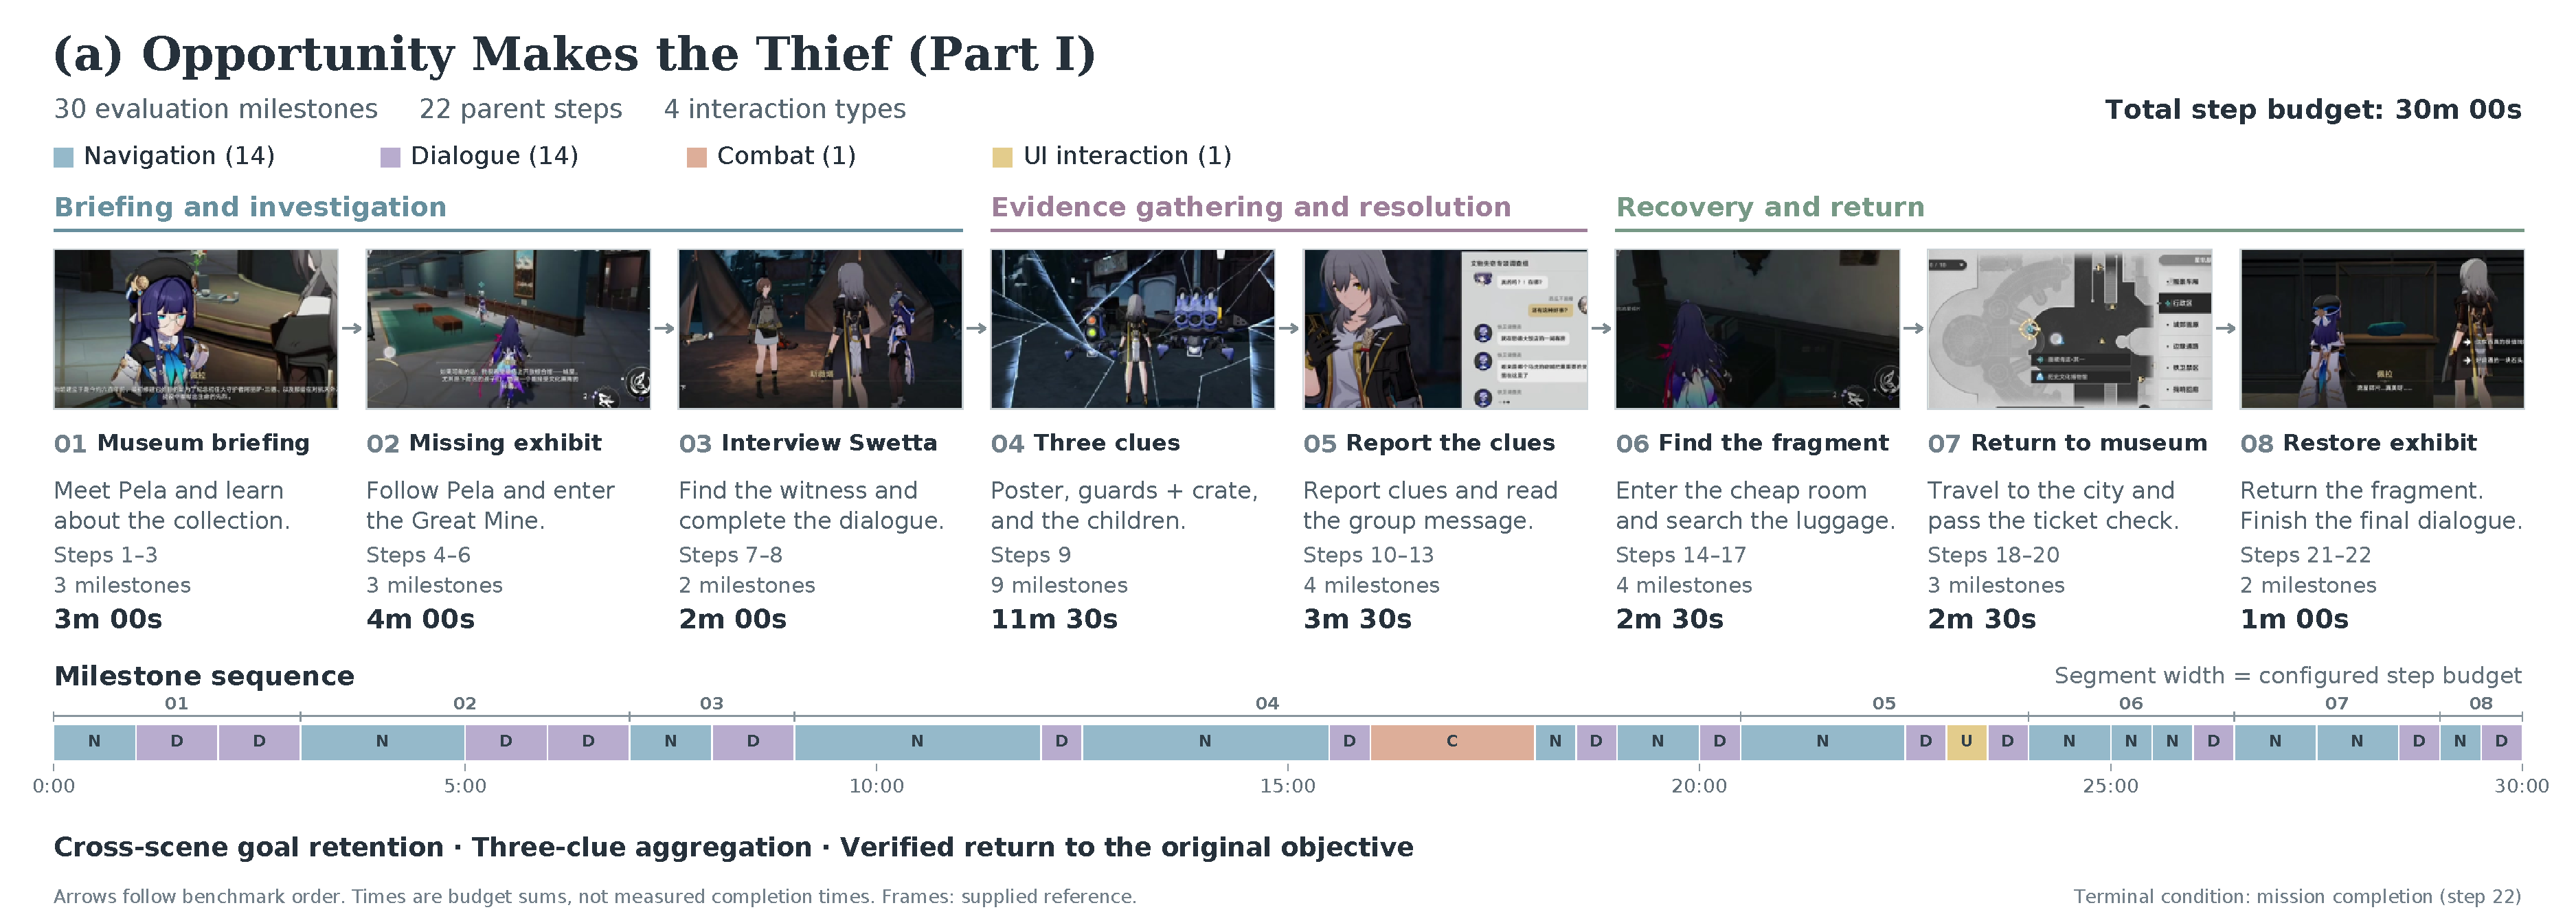
\includegraphics[width=\linewidth]{figs/hsr_sidequest_make_the_thief.pdf}
        \vspace{-2mm}
        \centerline{\textbf{(a) Opportunity Makes the Thief (Part \uppercase\expandafter{\romannumeral1})}}
    \end{minipage}
    \\
    \vspace{2mm}
    \begin{minipage}[t]{0.80\linewidth}
        \centering
        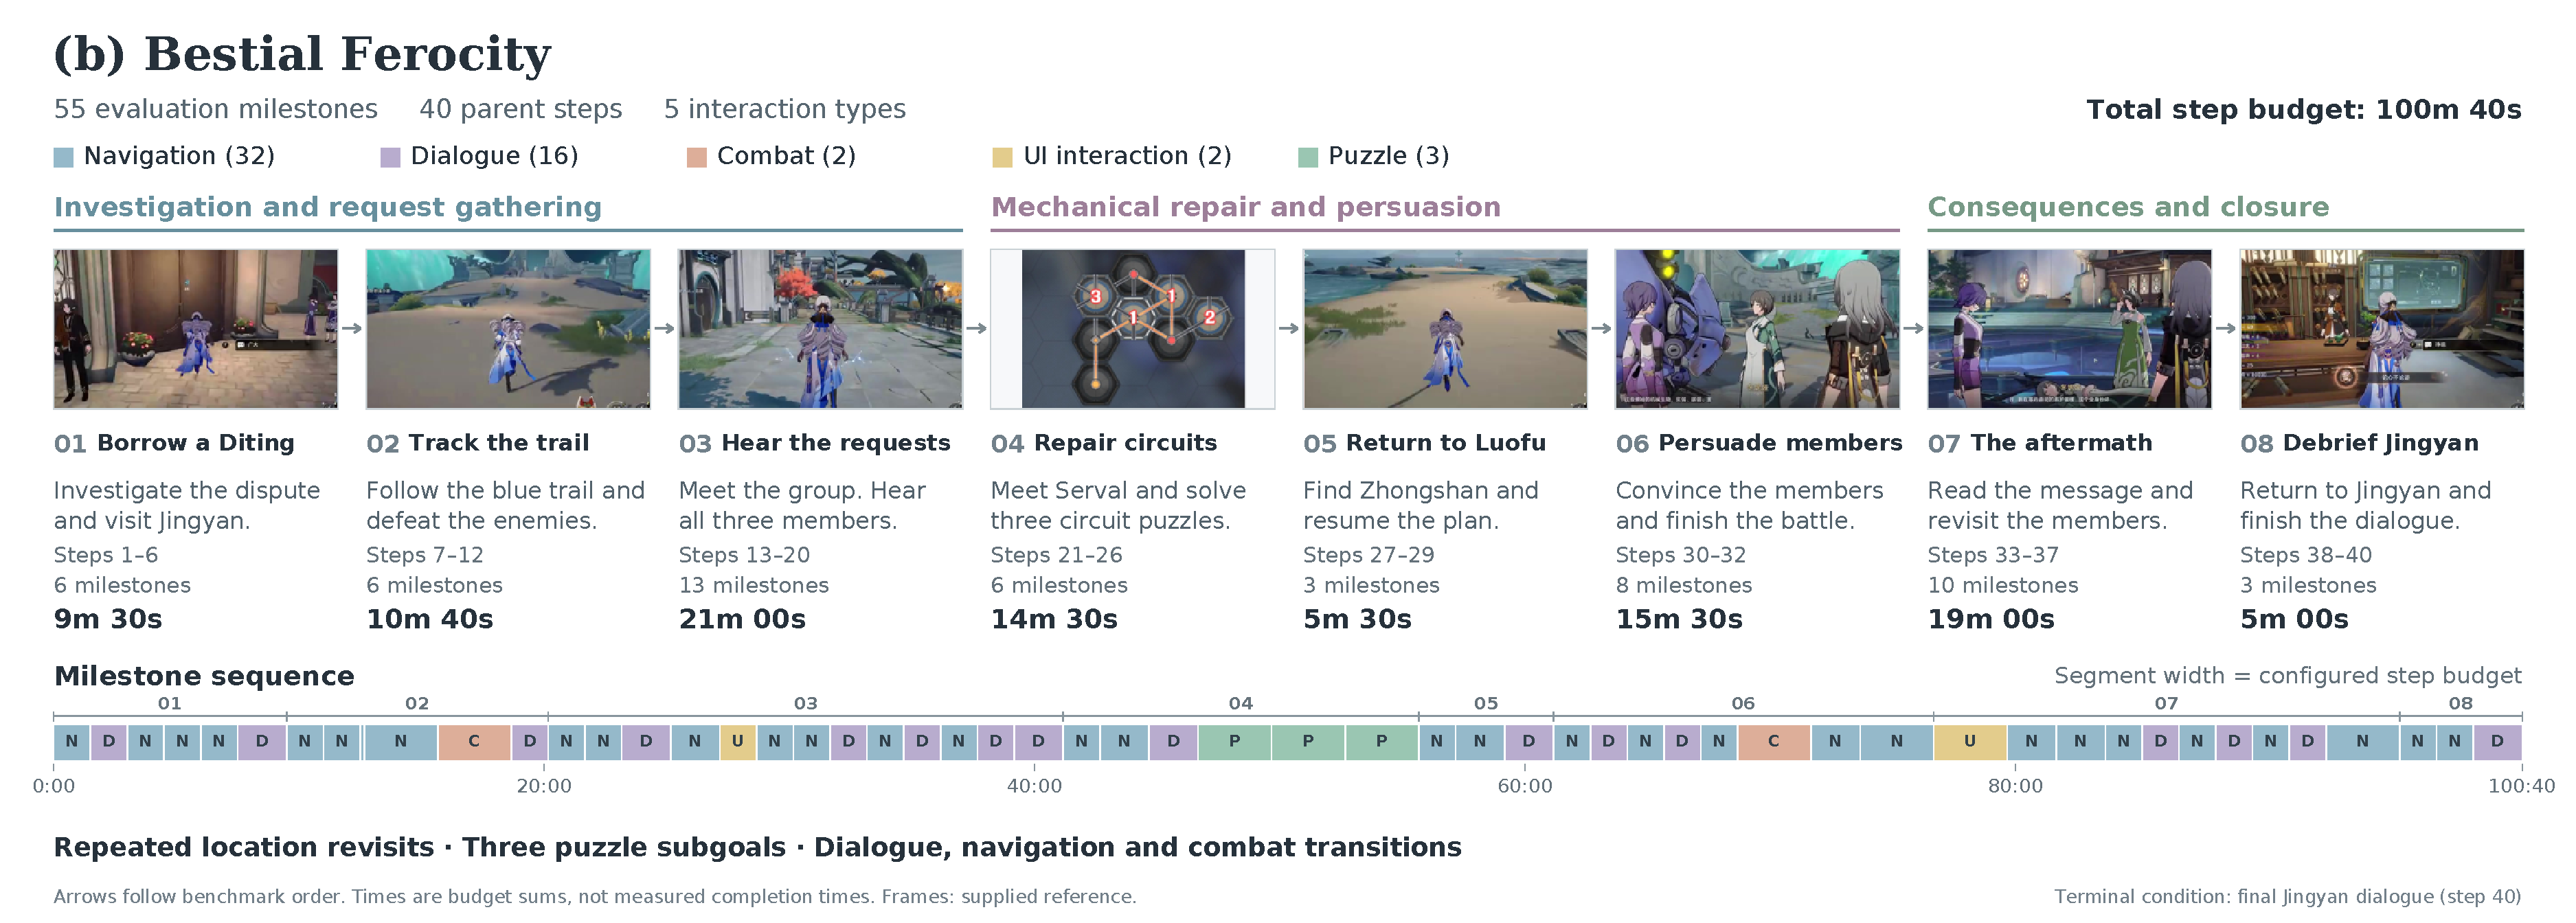
\includegraphics[width=\linewidth]{figs/hsr_sidequest_bestial_ferocity.pdf}
        \vspace{-2mm}
        \centerline{\textbf{(b) Bestial Ferocity}}
    \end{minipage}
    \caption{
    \textbf{Representative long-horizon side quests in the Honkai: Star Rail evaluation suite.}
  (a) Opportunity Makes the Thief (Part I) contains 30 milestones with navigation, dialogue, combat, and UI interaction. (b) Bestial
Ferocity contains 55 milestones and additionally includes three mechanical-repair puzzles. Both panels show ordered milestone sequences and configured step budgets rather than measured completion times.
    }
    \label{fig:hsr_sidequests}
\end{figure*}

\begin{figure*}[!htbp]
    \centering
    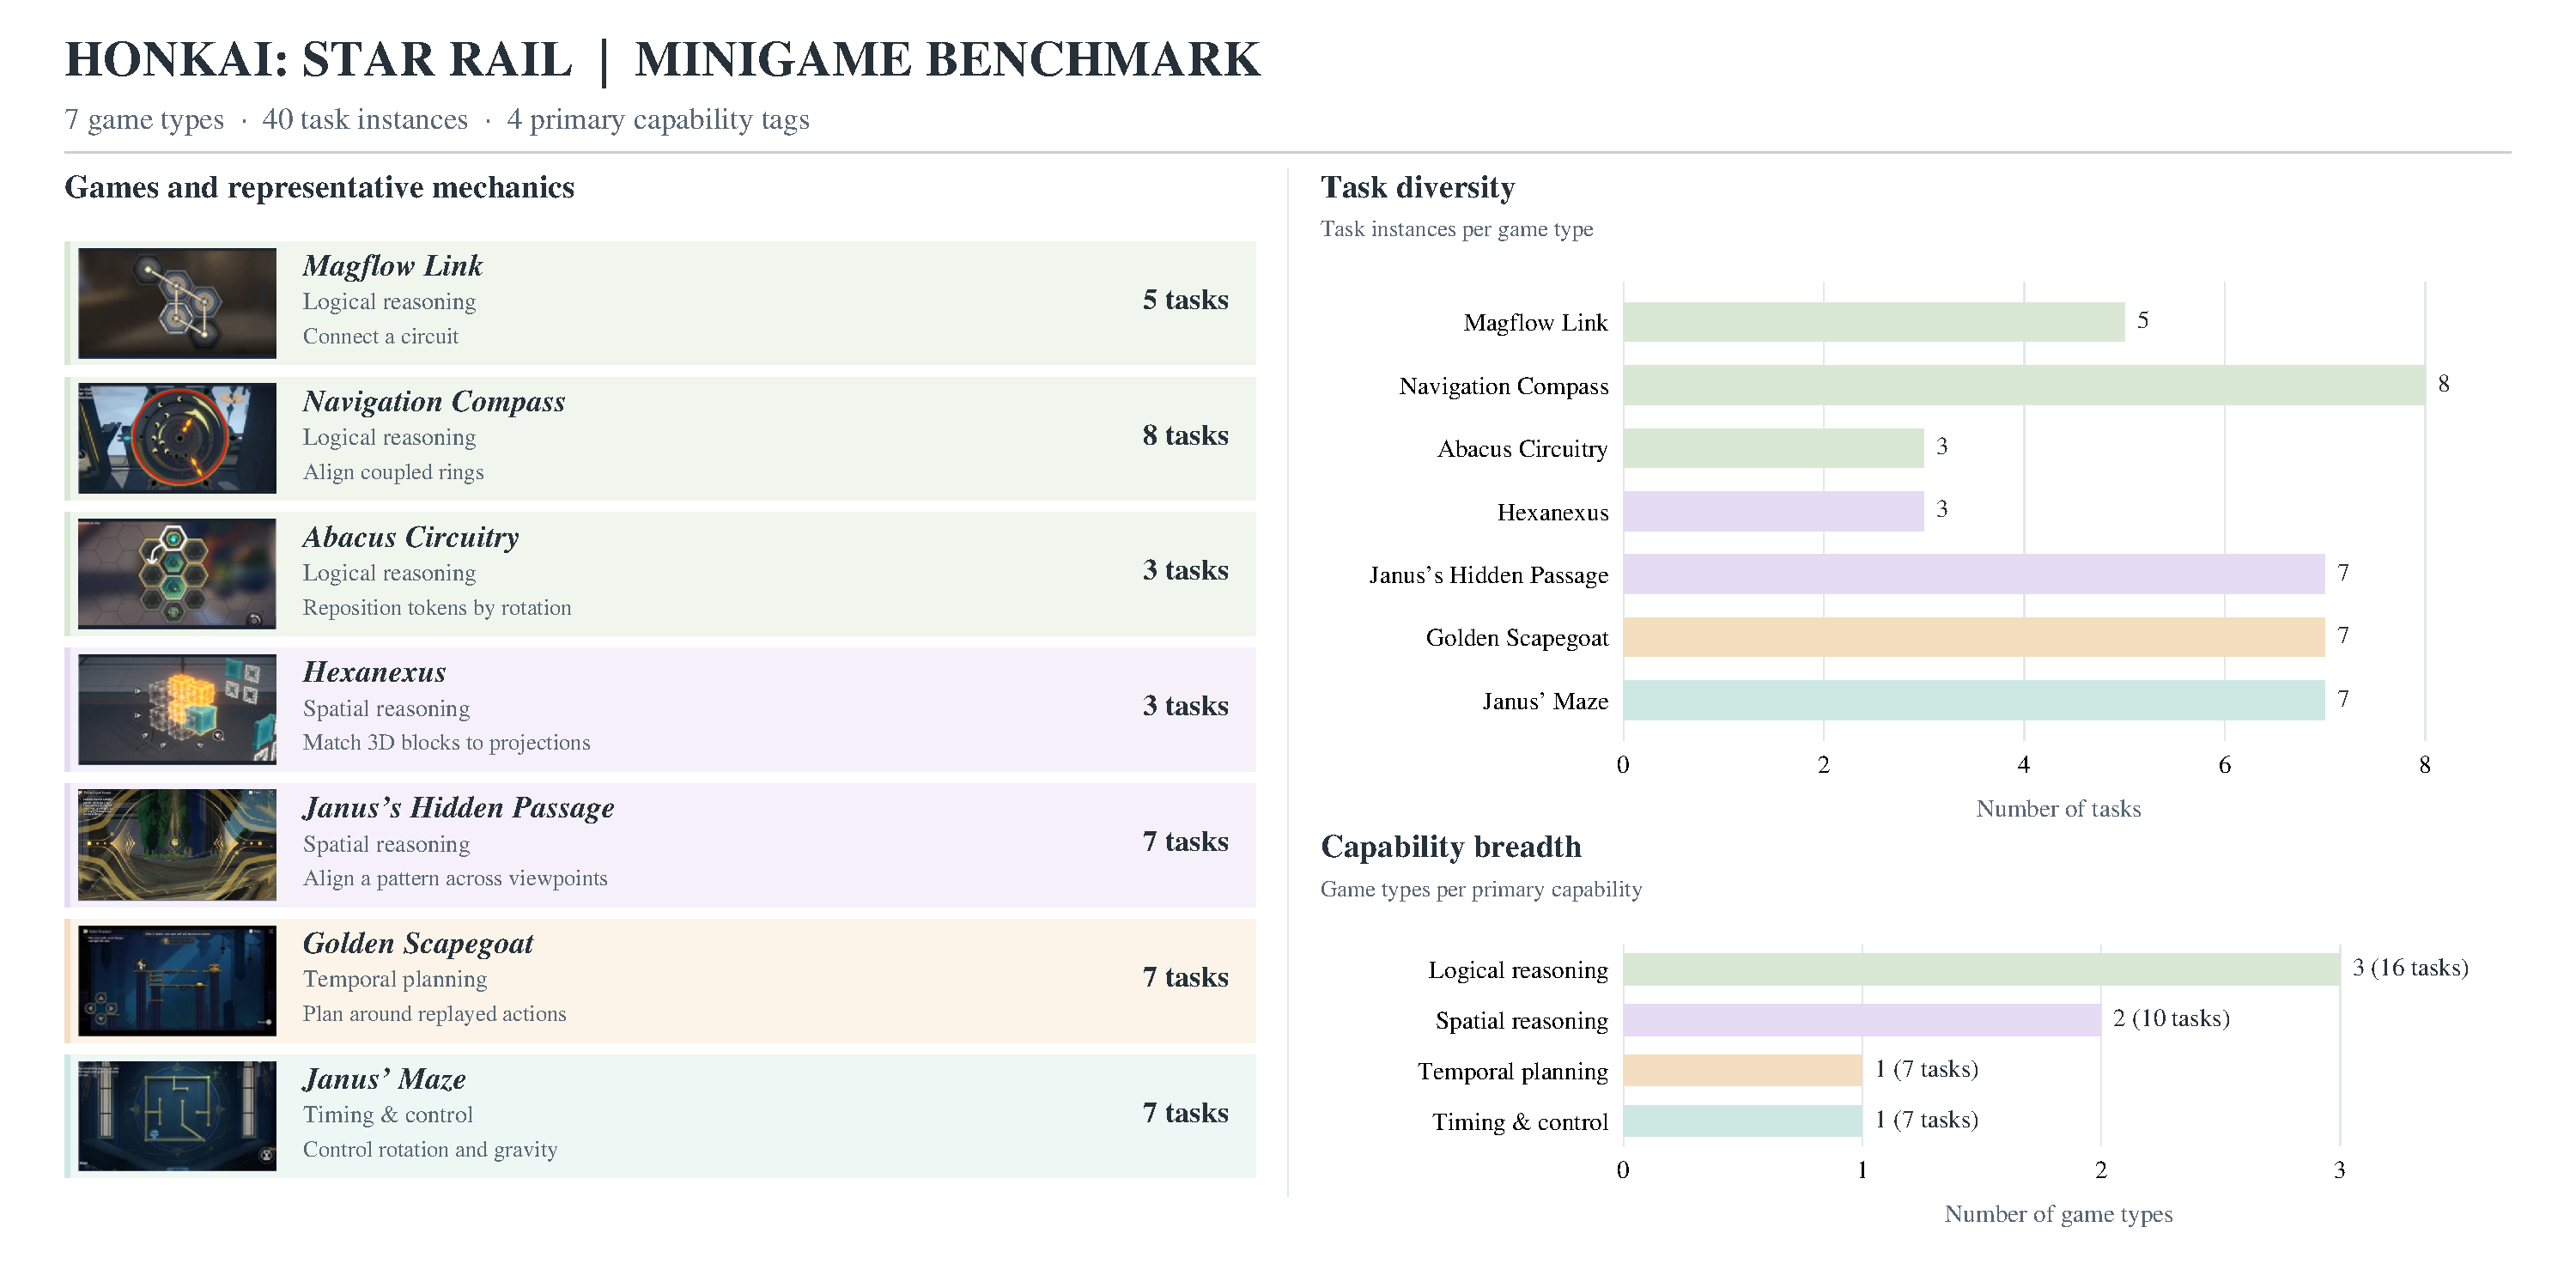
\includegraphics[width=0.87\linewidth]{figs/hsr_minigame_bench.pdf}
    \caption{
    \textbf{Overview of the minigame benchmark in the Honkai: Star Rail evaluation suite.} The benchmark contains 40 task instances across seven game types. The left panel shows representative gameplay examples, instance counts, and mechanics. The upper-right chart shows the number of instances per type, while the lower-right chart groups minigames by four descriptive primary capability tags, with instance totals in parentheses. Each minigame type is assigned one primary tag for counting and may require additional abilities. Screenshots illustrate game types and are not necessarily drawn from the evaluated instances.
    }
    \label{fig:hsr_minigames}
\end{figure*}

The second subset contains 40 instances across 7 \textbf{minigame} types, covering pattern composition, logical reasoning, spatial reasoning, temporal planning, and timing-sensitive control. Each type contains between one and sixteen evaluated instances. Figure~\ref{fig:hsr_minigames} illustrates the minigame mechanics and instance distribution. We report the success rates for each type and compute overall accuracy as the unweighted mean of the seven type-level rates. Each type therefore contributes equally, regardless of its number of instances. Per-instance evaluation and taxonomy are described in Appendix~\ref{app:hsr_protocol}.


\subsection{Scaling Cross-Game Control with CPT}
\label{sec:exp_cpt_scaling}

\subsubsection{Controlled Scaling Setup}

The controlled study in GameScaling \cite{gamescaling} examines how model size, gameplay budget, and game composition affect CPT performance and cross-game generalization. These results guide further HSR-augmented \ourmodel-CPT recipes. We summarize its experimental setup here.

As summarized in Table~\ref{tab:cpt_scaling_setup}, the study comprises $4\times6\times5=120$ configurations spanning Qwen3.5 backbone sizes, gameplay budgets, and data mixtures. All other training settings are held fixed. Across configurations, gameplay trajectories account for 85\% of training tokens, while the remaining 15\% come from a fixed pool of general multimodal data. The five mixtures, S1--S5, vary only the composition of the gameplay portion: Minecraft accounts for 100\%, 51.4\%, 27.1\%, 2.8\%, and 0\%, respectively. The remaining gameplay data in S2--S5 are sampled from the same multi-game pool.


\begin{table}[t]
    \centering
    \small
    \setlength{\tabcolsep}{4pt}
    \renewcommand{\arraystretch}{1.08}
    \begin{tabular}{p{0.20\linewidth}p{0.40\linewidth}p{0.31\linewidth}}
        \toprule
        \textbf{Scaling Dimension}
        & \textbf{Controlled Configurations}
        & \textbf{Research Focus} \\
        \midrule
        Model size $N$
        & Qwen3.5 0.8B, 2B, 9B, 27B
        & Capacity and data efficiency \\
        
        Gameplay budget $D$
        & 50, 100, 200, 400, 800, 1,600 hours
        & Gains from additional interaction \\
        
        Game mixture
        & S1-S5
        & Effect of target-game coverage \\
        \bottomrule
    \end{tabular}
    \caption{
    \textbf{Experimental configurations for the GameScaling CPT study.} The study varies model size, gameplay budget, and game mixture across 120 configurations.
    }
    \label{tab:cpt_scaling_setup}
\end{table}


Let $w_{\mathrm{MC}}$ denote the Minecraft fraction of the gameplay mixture.
Consistent with Sec.~\ref{sec:cpt_scaling}, we use
$q=w_{\mathrm{MC}}$
for Minecraft validation loss, and
$q=1-w_{\mathrm{MC}}$
for validation over the multi-game training distribution.
The latter denotes the non-Minecraft fraction of the gameplay experience.


\subsubsection{Interface Adaptation and Scaling Behavior}

We summarize the interface-adaptation and scaling results reported in GameScaling~\cite{gamescaling}. The corresponding plots are provided in Appendix~\ref{app:gamescaling_results}.

\paragraph{Early CPT adapts the pretrained model to the shared control interface.}
Figure~\ref{fig:cpt_action_losses} shows that keyboard, mouse, and action-format losses decrease rapidly during the early stage of CPT, while directional prediction accuracy steadily improves.
Checkpoints trained for only 50 gameplay hours already reduce validation loss on both training and unseen games relative to their corresponding base models. This early improvement across distinct action components suggests that a substantial part of initial CPT learning concerns the mechanics of executable control. It also explains why interface adaptation can precede the larger gameplay-specific gains that emerge with additional interaction experience.


\paragraph{Later scaling gains increasingly depend on game composition.}
Figure~\ref{fig:cpt_scaling_losses} separates training fit from cross-game generalization.
Minecraft-heavy mixtures S1-S3 continue to reduce Minecraft validation loss as the interaction budget increases, while the low-Minecraft mixtures S4 and S5 tend to saturate.
On the remaining training games, multi-game mixtures continue to improve while Minecraft-only training eventually plateaus or degrades.
Adding the same amount of gameplay data can therefore produce different gains, depending on its coverage of the target distribution.

Larger models learn more efficiently early in training, but their gains still depend on data composition.
Under single-game training, stronger adaptation to Minecraft can coincide with degraded performance on other games.
Multi-game mixtures alleviate this effect.
For distant unseen games, validation loss typically improves during early interface adaptation and then plateaus or increases even while training loss continues to decrease.
These observations motivate considering model capacity, interaction budget, and target-game coverage jointly.


Evaluation results on game benchmarks complement the validation-loss analysis with executable gameplay outcomes. As shown in Figure~\ref{fig:cpt_benchmark_hours}, additional CPT experience generally improves performance in training-covered and behaviorally related environments, particularly at smaller model scales. The comparison across S1-S5 also shows why the amount of gameplay alone is an incomplete description of the training signal. Mixtures that expose the model to multiple interaction patterns provide broader coverage than single-game training and support transfer to related environments. For Gamer, these findings motivate scaling game diversity alongside data volume rather than treating all recorded gameplay hours as equally informative for every target game.

\subsubsection{Scaling-Law Fit and Predictive Range}

GameScaling~\cite{gamescaling} fits the empirical relation summarized in Sec.~\ref{sec:cpt_scaling},
\begin{equation}
\mathcal{L}_{\mathrm{val}}(N,D,q)
=
E
+
\frac{C_N}{N^a}
+
\frac{C_D q^\eta}{D^b}
+
\frac{C_q}{(q+\epsilon)^c},
\label{eq:exp_scaling_law}
\end{equation}
to characterize validation loss as a function of model size, gameplay budget, and target-dependent data composition.

The study reports that the standard model-and-data scaling relation fits training loss with $R^2=0.980$ and RMSE $=0.0041$.
For Minecraft and the multi-game training distribution, the composition-aware relation achieves the fit accuracy reported in Table~\ref{tab:scaling_fit}.

\begin{table}[t]
    \centering
    \small
    \setlength{\tabcolsep}{4pt}
    \begin{tabular}{lcccc}
        \toprule
        \textbf{Validation}
        & \textbf{$q$}
        & \textbf{$R^2$}
        & \textbf{RMSE}
        & \textbf{Within $R^2$} \\
        \midrule
        Minecraft
        & $w_{\mathrm{MC}}$
        & 0.982
        & 0.0020
        & 0.912 \\
        
        Training games
        & $1-w_{\mathrm{MC}}$
        & 0.995
        & 0.0012
        & 0.959 \\
        \bottomrule
    \end{tabular}
    \caption{
    \textbf{Fit accuracy of the composition-aware scaling relation.}
    Within-mixture $R^2$ measures variation explained by model size and data budget after removing mean differences across mixtures.
    }
    \label{tab:scaling_fit}
\end{table}

Both validation distributions yield a positive fitted $\eta$. At a fixed model size, increasing the interaction budget therefore produces larger gains when the training mixture contains more experience relevant to the validation distribution. The fit captures the same interaction between data quantity and composition visible in the measured curves. In particular, it distinguishes a model that has seen more gameplay from one that has seen more gameplay relevant to the target environment. This provides a practical basis for choosing CPT mixtures when expanding the training corpus.

GameScaling further performs block-wise holdout tests over model sizes, data budgets, and game mixtures.
Capacity and budget holdouts support prediction within the measured range.
Mixture prediction is more sensitive to the availability of nearby compositions.
The fitted relation summarizes the observed scaling regime across the evaluated distributions.
Fitting details and holdout results are provided in Appendix~\ref{app:cpt_scaling_fit}.

Distant unseen games provide a useful negative control.
Their validation loss rises again after early adaptation.
Fitting the same functional form yields a data exponent close to $b=0$.
The nominal $R^2=0.855$ is dominated by static differences across mixtures, while the within-mixture $R^2$ is only 0.079.
A high overall fit score therefore does not imply continued improvement from additional interaction data.


\subsubsection{Cross-Game Performance of CPT Policies}


While the controlled GameScaling study reveals how model size and gameplay data affect CPT, an important question remains: whether CPT can translate general-purpose visual understanding into executable control across diverse games. Unlike static visual reasoning, gameplay requires the agent to continuously interpret observations, execute precise actions, and adapt to evolving environments. We therefore evaluate whether CPT-trained policies can achieve effective real-time control across different games and backbone architectures. Table~\ref{tab:cpt_game_benchmarks} compares two CPT checkpoints, initialized from Qwen3-VL-8B Dense and Qwen3.5-35B-A3B MoE, with general-purpose multimodal baselines on four public game benchmarks. We report real-time (RT) scores as the primary results, together with their signed differences from time-paused (TP) evaluation.


\begin{table*}[t]
\centering
\small
\setlength{\tabcolsep}{4.5pt}
\renewcommand{\arraystretch}{1.06}
\caption{
\textbf{Cross-game performance of CPT policies under real-time interaction.}
The final two rows report CPT checkpoints based on Qwen3-VL-8B Dense and Qwen3.5-35B-A3B MoE. The main value is the real-time (RT) score, while parentheses show its difference from idealized time-paused (TP) evaluation, computed as RT$-$TP. Green indicates a positive difference, red a negative difference, and zero denotes no change. Higher scores are better. The performance of controlled GameScaling-S3 checkpoints is not included in this table.
}
\label{tab:cpt_game_benchmarks}

\resizebox{0.92\linewidth}{!}{
\begin{tabular}{lccccc}
\toprule
\textbf{Model}
& \textbf{MCU $\uparrow$}
& \textbf{ViZDoom $\uparrow$}
& \textbf{OmniGameArena $\uparrow$}
& \textbf{GameWorld $\uparrow$}
& \textbf{Average $\uparrow$} \\
\midrule

GPT-5.6-Sol
& 8.7 (\textcolor{red}{$-$73.3})
& 2.7 (\textcolor{red}{$-$24.0})
& 14.5 (\textcolor{red}{$-$31.1})
& 44.3 (\textcolor{red}{$-$9.6})
& 17.6 (\textcolor{red}{$-$34.5}) \\

GPT-5.6-Luna
& 5.3 (\textcolor{red}{$-$48.7})
& 2.9 (\textcolor{red}{$-$21.2})
& 13.2 (\textcolor{red}{$-$13.5})
& 41.6 (\textcolor{red}{$-$3.3})
& 15.8 (\textcolor{red}{$-$21.6}) \\

Claude-Opus-5.0
& 8.7 (\textcolor{red}{$-$48.0})
& 2.0 (\textcolor{red}{$-$18.8})
& 16.4 (\textcolor{red}{$-$28.0})
& 42.0 (\textcolor{red}{$-$10.8})
& 17.3 (\textcolor{red}{$-$26.4}) \\

GLM-5.3-Flash
& 7.3 (\textcolor{red}{$-$40.0})
& 1.9 (\textcolor{red}{$-$17.0})
& 12.3 (\textcolor{red}{$-$11.2})
& 29.6 (\textcolor{red}{$-$4.4})
& 12.8 (\textcolor{red}{$-$18.1}) \\

DeepSeek-V4-Flash-Vision
& 7.3 (\textcolor{red}{$-$28.7})
& 3.3 (\textcolor{red}{$-$9.7})
& 11.6 (\textcolor{red}{$-$15.5})
& 28.5 (\textcolor{red}{$-$13.3})
& 12.7 (\textcolor{red}{$-$16.8}) \\

\midrule

Qwen3.5-0.8B
& 0.0 ($+$0.0)
& 1.0 (\textcolor{green}{$+$0.1})
& 1.8 (\textcolor{green}{$+$0.1})
& 15.1 (\textcolor{green}{$+$1.3})
& 4.5 (\textcolor{green}{$+$0.4}) \\

Qwen3.5-2B
& 0.0 ($+$0.0)
& 1.5 (\textcolor{green}{$+$0.6})
& 1.7 (\textcolor{red}{$-$0.1})
& 16.3 (\textcolor{red}{$-$3.5})
& 4.9 (\textcolor{red}{$-$0.7}) \\

Qwen3.5-9B
& 3.3 ($+$0.0)
& 3.2 (\textcolor{green}{$+$0.4})
& 4.1 (\textcolor{red}{$-$1.1})
& 27.7 (\textcolor{red}{$-$1.5})
& 9.6 (\textcolor{red}{$-$0.5}) \\


Qwen3.5-27B
& 4.0 (\textcolor{red}{$-$5.3})
& 2.9 (\textcolor{red}{$-$2.7})
& 7.6 (\textcolor{red}{$-$2.1})
& 25.2 (\textcolor{red}{$-$4.1})
& 9.9 (\textcolor{red}{$-$3.6}) \\


\midrule

\ourmodel-8B-CPT
& 47.7 (\textcolor{red}{$-$13.0})
& 14.4 (\textcolor{red}{$-$2.2})
& 21.9 (\textcolor{red}{$-$3.0})
& 34.0 (\textcolor{green}{$+$0.7})
&  29.5 (\textcolor{red}{$-$4.4})\\

\ourmodel-35B-A3B-CPT
& 65.3 (\textcolor{green}{$+$18.6})
& 11.9 (\textcolor{green}{$+$1.7})
& 18.7 (\textcolor{red}{$-$6.7})
& 30.2 (\textcolor{red}{$-$0.1})
&  31.5 (\textcolor{green}{$+$3.4}) \\

\bottomrule
\end{tabular}
}
\end{table*}

\textbf{CPT supports effective cross-game control across Dense and MoE backbones.}
The Qwen3-VL-8B CPT policy achieves an average real-time score of 29.5, while the Qwen3.5-35B-A3B MoE CPT policy reaches 31.5. Both exceed the strongest listed general-purpose baseline. The difference is especially clear on MCU, where the two CPT policies score 47.7 and 65.3, respectively. Their results also show complementary strengths across games. The 8B Dense policy achieves 21.9 on OmniGameArena and 34.0 on GameWorld, while the MoE policy performs particularly strongly on MCU. These results extend the scaling analysis from action prediction and validation loss to executable gameplay, and show that the CPT approach is applicable to both Dense and MoE model architectures.



\textbf{Real-time evaluation provides a practical measure of control ability.} The paired RT and TP results further highlight the importance of real-time inference for interactive game control. While most general-purpose models experience substantial performance degradation when the game continues advancing during inference, our 8B CPT policy shows only a modest decrease, demonstrating its ability to maintain effective control under real-time constraints. Notably, the MoE CPT policy achieves an average RT--TP improvement of +3.4 points. This positive gain is consistent with its faster inference, which enables more timely interaction with the evolving environment and reduces the accumulation of control errors. These results suggest that low-latency inference is important not only for preserving gameplay performance but also for fully realizing the capabilities learned through CPT. Further details and results of the 120-configuration GameScaling study are provided in \citet{gamescaling}. Table~\ref{tab:cpt_game_benchmarks} complements the scaling analysis with direct evidence of executable cross-game control. We further investigate the inference optimizations enabling real-time interaction in Sec.~\ref{sec:exp_streaming}.


% \subsection{SFT for Long-Horizon Instruction Following and Gameplay Generalization}
% \label{sec:exp_sft}
\begin{table*}[!ht]
\centering
\caption{
\textbf{Long-horizon instruction following across two side quests.}
To improve evaluation robustness, we evaluate each task three times and report the averaged success rate (\%) of evaluated tasks for each interaction type.
Overall accuracy (Acc) divides successful task executions by all evaluated task
executions, pooling repeated attempts over the 30 or 55 milestone units.
Opportunity Makes the Thief (Part I) and Bestial Ferocity contain
30 and 55 milestones, respectively.
}
\label{tab:sidequest_results}

\setlength{\tabcolsep}{4pt}
\renewcommand{\arraystretch}{1.12}

\resizebox{0.92\linewidth}{!}{%
\begin{tabular}{l*{11}{c}}
\toprule

\multirow{2}{*}{\textbf{Model}}
& \multicolumn{5}{c}{\textbf{Opportunity Makes the Thief (I)}}
& \multicolumn{6}{c}{\textbf{Bestial Ferocity}} \\

\cmidrule(lr){2-6}
\cmidrule(lr){7-12}

& Nav.
& Dialogue
& Combat
& UI
& \textbf{Acc $\uparrow$}
& Nav.
& Dialogue
& Combat
& UI
& Puzzle
& \textbf{Acc $\uparrow$} \\


\midrule

Gemini-3.8-Flash
& 0.0 & 35.7 & 0.0 & 0.0 & 16.7
& 31.2 & 81.2 & 50.0 & 50.0 & 0.0 & 45.5 \\

GPT-5.6-Sol
& 7.1 & 28.6 & 0.0 & 0.0 & 16.7
& 28.1 & 68.8 & 50.0 & 100.0 & 0.0 & 41.8 \\

GPT-5.6-Luna
& 7.1 & 14.3 & 0.0 & 0.0 & 10.0
& 18.8 & 43.8 & 0.0 & 0.0 & 0.0 & 23.6 \\

Claude-Opus-5.0
& 7.1 & 21.4 & 0.0 & 0.0 & 13.3
& 15.6 & 56.2 & 50.0 & 50.0 & 0.0 & 29.1 \\

GLM-5.3-Flash
& 7.1 & 21.4 & 0.0 & 0.0 & 13.3
& 15.6 & 43.8 & 50.0 & 0.0 & 0.0 & 23.6 \\

DeepSeek-V4-Flash-Vision
& 14.3 & 35.7 & 0.0 & 0.0
& 23.3
& 15.6 & 56.2 & 50.0 & 0.0 & 0.0 & 27.3 \\

\midrule

Qwen3-VL-8B (Base)
& 0.0 & 0.0 & 0.0 & 0.0 & 0.0
& 12.5 & 18.8 & 33.3 & 0.0 & 0.0 & 13.9 \\

\ourmodel-CPT
& 14.3 & 50.0 & 100.0 & 33.3 & 34.4
& 36.5 & 70.8 & 100.0 & 66.7 & 0.0 & 47.9 \\

\ourmodel-SFT
& 47.6 & \textbf{92.9} & 100.0 & 100.0 & 72.2
& 55.2 & 97.9 & 100.0 & 100.0 & \textbf{22.2} & 69.1 \\

\textbf{\ourmodel-RL}
& \textbf{69.1} & 88.1 & \textbf{100.0} & \textbf{100.0} & \textbf{80.0}
& \textbf{80.2} & \textbf{100.0} & \textbf{100.0} & \textbf{100.0} & 11.1 & \textbf{83.6} \\

\bottomrule
\end{tabular}%
}
\end{table*}

\subsection{Long-Horizon Instruction Following in Side Quests}
\label{sec:exp_sft}
\label{sec:exp_rl}

The two side quests require the agent to carry out multi-stage tasks while retaining information from earlier interactions. Table~\ref{tab:sidequest_results} reports verified task-execution success rates on \ourmodel.

\textbf{SFT substantially improves long-horizon task execution.}
On \emph{Opportunity Makes the Thief (Part I)}, overall accuracy increases from 0.0\% for Qwen3-VL-8B to 34.4\% after HSR-augmented CPT and 72.2\% after SFT. On \emph{Bestial Ferocity}, the corresponding scores are 13.9\%, 47.9\%, and 69.1\%. Thus, SFT adds 37.8 and 21.2 percentage points over the respective CPT checkpoints. The improvement is visible across distinct interaction types. For example, navigation rises from 14.3\% to 47.6\% on the first quest, while dialogue increases from 70.8\% to 97.9\% on the second. These outcomes are consistent with the objective of multi-level instruction tuning, which trains the same action policy to follow goals that span local operations, intermediate subgoals, and longer task sequences.

Both quests involve repeated scene transitions, UI interactions, and changes in objectives. To make progress, the agent must retain relevant information from earlier interactions and use it to decide what to do next. SFT improves performance on held-out tasks, suggesting that task-conditioned reasoning and memory can support this behavior in a familiar game, even when the specific evaluation objectives were excluded from training.

\textbf{Online RL further strengthens long-horizon execution.}
We perform online RL on the basis of the SFT checkpoint. Relative to its SFT initialization, TA-GRPO improves overall task-execution accuracy from 72.2\% to 80.0\% on \emph{Opportunity Makes the Thief (Part I)} and from 69.1\% to 83.6\% on \emph{Bestial Ferocity}. These correspond to gains of \textbf{7.8} and \textbf{14.5 percentage points}, respectively. Navigation accuracy rises from 47.6\% to 69.1\% on the first quest and from 55.2\% to 80.2\% on the second. On \emph{Bestial Ferocity}, dialogue reaches 100\% after RL. These results suggest that verified interaction feedback helps refine the policy's ability to advance toward task goals over extended trajectories.

The gains across both side quests highlight the complementary roles of instruction supervision and online policy optimization. SFT provides task-conditioned decisions and memory, while RL allows the policy to learn from the consequences of its own actions under game-native verification. Importantly, these improvements are obtained without changing the underlying action interface or model architecture. Appendix~\ref{app:rl_rollouts} provides representative training and held-out development rollouts that illustrate how navigation and final-target interactions evolve across checkpoints.


\begin{table*}[t]
\centering
\caption{
\textbf{Instruction generalization across seven minigame types.}
To improve evaluation robustness, we evaluate each task three times and report the averaged task success rates (\%) on a reduced benchmark of 40 task instances.
Each task score is the mean of its valid evaluation attempts.
Acc is the unweighted average across the seven game types.
ML, NC, AC, HX, JHP, GS, and JM denote Magflow Link, Navigation Compass,
Abacus Circuitry, Hexanexus, Janus's Hidden Passage, Golden Scapegoat,
and Janus's Maze, respectively.
}
\label{tab:minigame_results}
\vspace{4pt}
\setlength{\tabcolsep}{6pt}
\renewcommand{\arraystretch}{1.12}
\resizebox{0.75\linewidth}{!}{%
\begin{tabular}{l*{8}{c}}
\toprule
\multirow{2}{*}{\textbf{Model}} & \multicolumn{7}{c}{\textbf{Minigame Types}} & \multirow{2}{*}{\textbf{Acc $\uparrow$}} \\
\cmidrule(lr){2-8}
& ML & NC & AC & HX & JHP & GS & JM & \\
\midrule
GPT-6.1-Sol & 20.0 & 37.5 & 0.0 & 33.3 & 14.3 & 0.0 & 14.3 & 17.1 \\
Gemini-3.8-Flash & 0.0 & 0.0 & 0.0 & 0.0 & 0.0 & 0.0 & 14.3 & 2.0 \\
GPT-5.6-Sol & 0.0 & 12.5 & 0.0 & 0.0 & 57.1 & 0.0 & 14.3 & 12.0 \\
GPT-5.6-Luna & 0.0 & 37.5 & 0.0 & 0.0 & 28.6 & 0.0 & 14.3 & 11.5 \\
Claude-Opus-5.0 & 0.0 & 12.5 & 0.0 & 0.0 & 57.1 & 0.0 & 0.0 & 9.9 \\
GLM-5.3-Flash & 0.0 & 0.0 & 0.0 & 0.0 & 57.1 & 0.0 & 0.0 & 8.2 \\
DeepSeek-V4-Flash-Vision & 0.0 & 0.0 & 0.0 & 0.0 & 0.0 & 0.0 & 14.3 & 2.0 \\
\midrule
Qwen3-VL-8B (Base)
& 0.0 & 8.3 & 0.0 & 0.0
& 0.0 & 4.8 & 9.5 & 3.2 \\

\ourmodel-CPT
& 20.0 & 37.5 & 0.0 & 0.0
& 23.8 & 9.5 & 14.3 & 15.0 \\

\ourmodel-SFT
& 40.0 & 50.0
& 11.1 & 11.1
& 76.2 & 33.3
& \textbf{52.4} & 39.2 \\

\textbf{\ourmodel-RL}
& \textbf{53.3} & \textbf{95.8}
& \textbf{22.2} & \textbf{33.3}
& \textbf{81.0} & \textbf{38.1}
& 23.8 & \textbf{49.7} \\
\bottomrule
\end{tabular}%
}
\end{table*}

\subsection{Instruction Generalization across Diverse Minigames}
\label{sec:exp_minigames}

The minigame suite emphasizes instruction following across different gameplay mechanics. This broader coverage is important because the tasks require different combinations of spatial reasoning, rule interpretation, visual matching, and device-level interaction rather than a single repeated control routine. Table~\ref{tab:minigame_results} reports success for each of the seven types and their unweighted macro-average.


\textbf{Instruction tuning broadens success across distinct minigame mechanics.}
The seven-type macro-average increases from 3.2\% for the base Qwen3-VL-8B to 15.0\% for \ourmodel-CPT and 39.2\% for \ourmodel-SFT, a further gain of 24.2 percentage points after instruction tuning. SFT reaches 76.2\% on Janus's Hidden Passage, 52.4\% on Janus's Maze, and 50.0\% on Navigation Compass. It also obtains non-zero mean success in all seven types, compared with three for the base model. The CPT checkpoint already improves the macro-average, providing a useful foundation for responding to gameplay observations and actions. SFT then connects these control capabilities to task-specific goals, which is reflected in improvements across puzzles with different interfaces and completion rules. The evaluation tasks are held out from training, so the comparison measures generalization to new instances and objectives within HSR.

\textbf{Online RL further improves performance across diverse mechanics.}
Following SFT, \ourmodel-RL raises the seven-type macro-average from 39.2\% to \textbf{49.7\%}, an additional gain of \textbf{10.5 percentage points}. The improvement is particularly pronounced on Navigation Compass, where accuracy increases from 50.0\% to 95.8\%. RL also improves Magflow Link from 40.0\% to 53.3\%, Hexanexus from 11.1\% to 33.3\% and Janus’s Hidden Passage from 76.2\% to 81.0\%, with additional gains on Abacus Circuitry and Golden Scapegoat. These results extend the benefits of online policy optimization beyond long-horizon quests to tasks involving diverse rules and interaction patterns. Together, the CPT, SFT, and RL stages progressively improve the model's ability to interpret instructions and execute actions across different game mechanics.

To prevent game types with more tasks from dominating the aggregate, the overall metric first averages attempts within each task and then gives each of the seven types equal weight. This makes the reported improvement a measure of breadth across mechanics rather than only the most frequent minigame.


\subsection{Impact of Real-Time Rollouts on Online RL}
\label{sec:exp_realtime_rl}

\textbf{Real-time interaction is critical for online RL in modern games.}
Unlike lightweight simulators, modern games involve continuously evolving environments, complex gameplay mechanics, and state-dependent interactions. In this setting, inference latency affects not only the responsiveness of the deployed agent but also the quality and efficiency of online policy learning. Delayed control can cause subsequent actions to operate on outdated observations, making it harder to obtain timely feedback from the environment. We therefore examine the effect of rollout frequency on RL training, comparing real-time Streaming-vLLM against standard vLLM rollouts. The game continues to advance under both settings.


\begin{figure*}[!htbp]
    \centering
    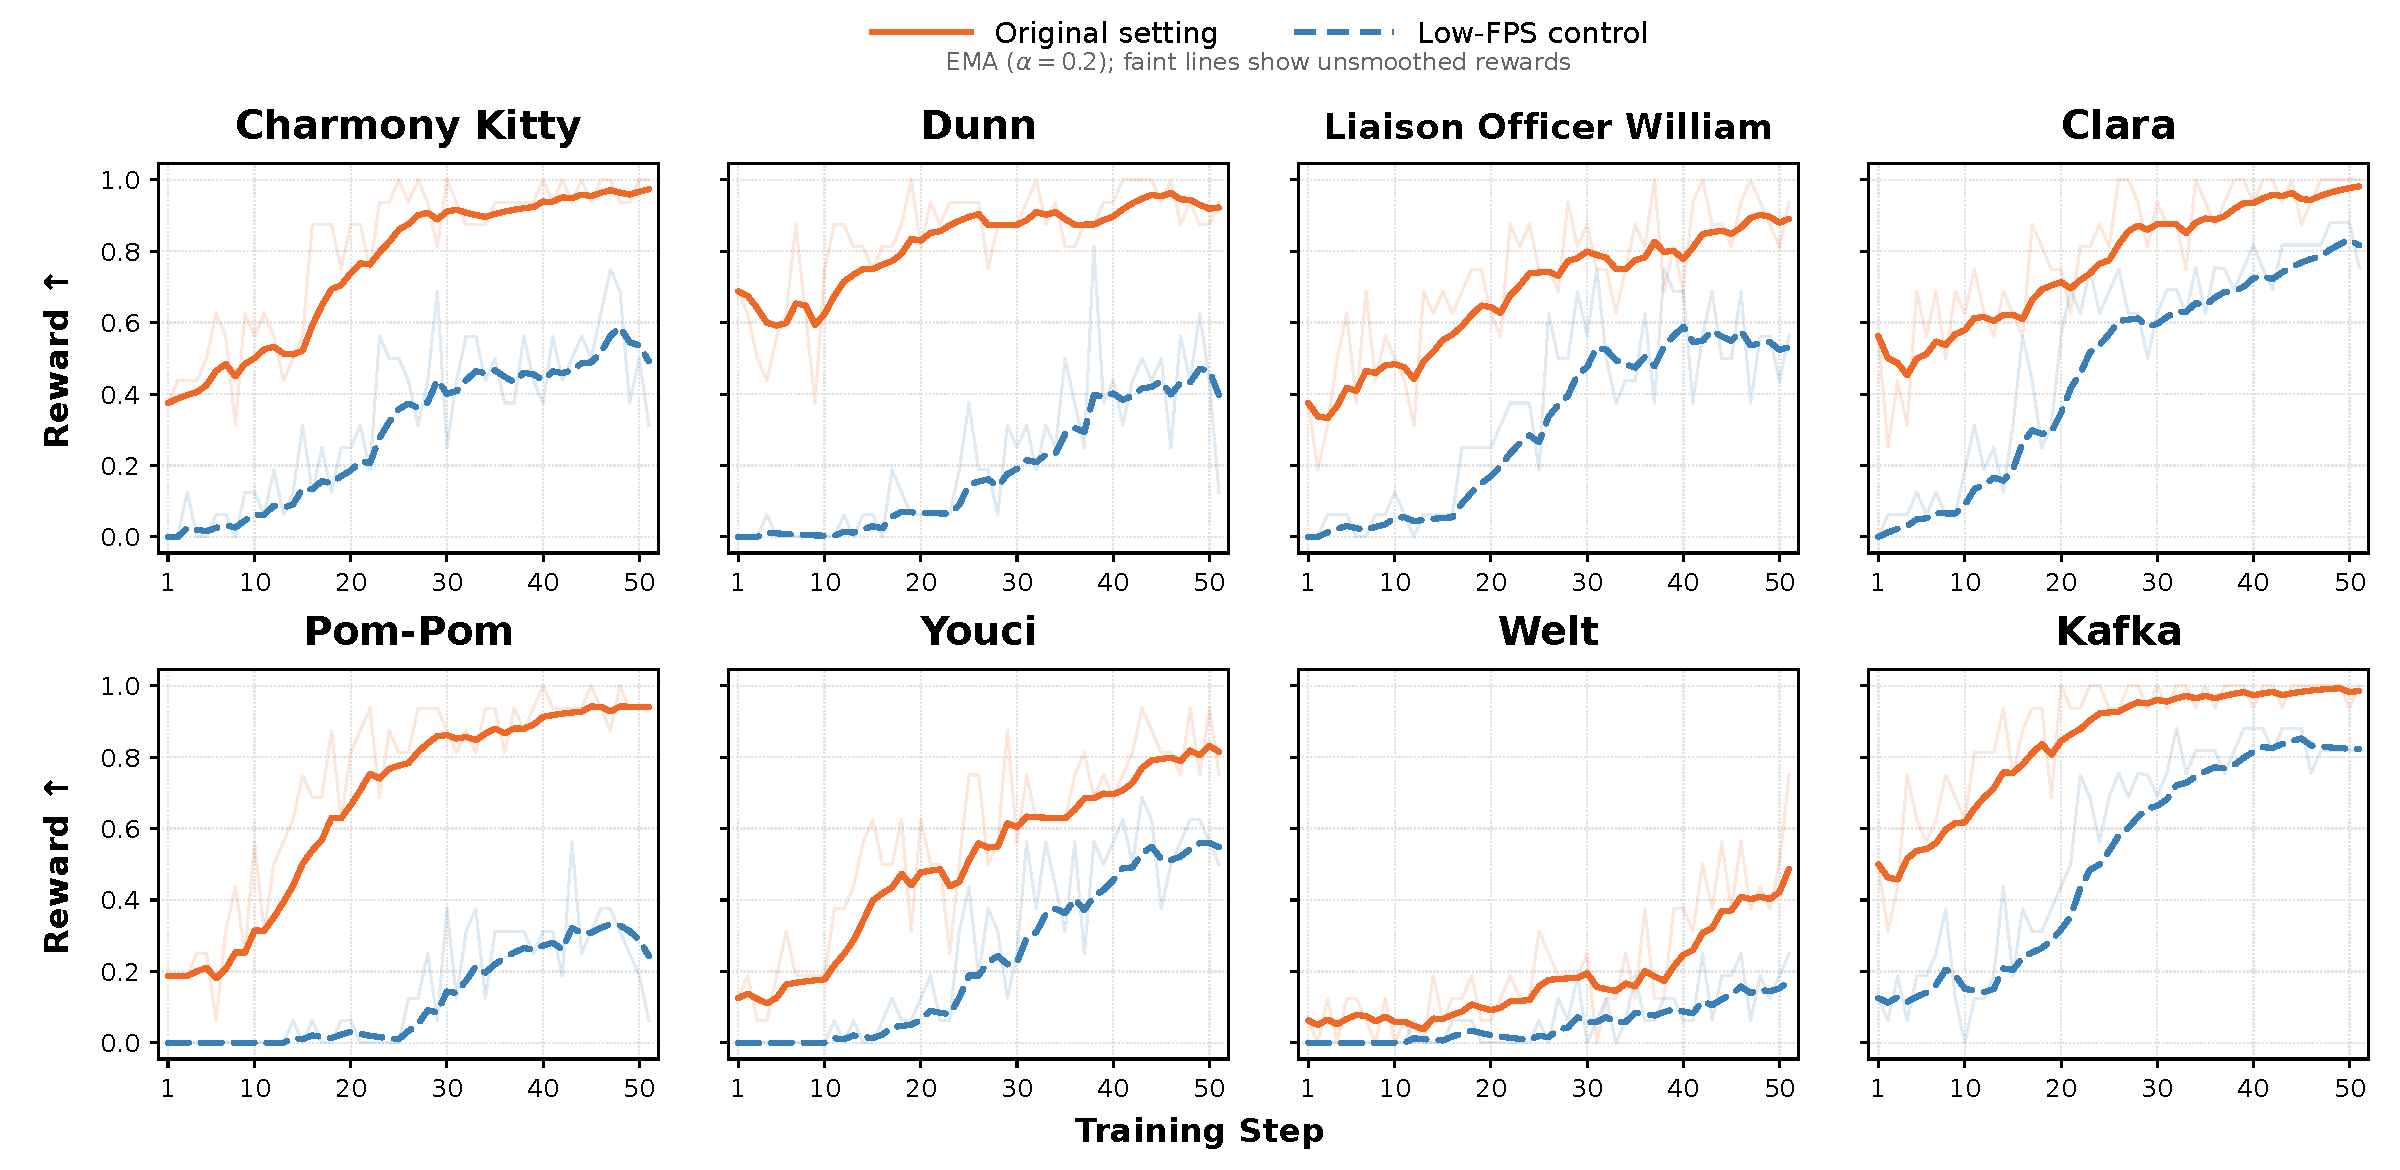
\includegraphics[width=0.85\linewidth]{figs/rl_reward_nav.pdf}
    \caption{\textbf{Real-time inference improves online RL learning across eight navigation tasks.} Task labels indicate navigation targets. For example, ``Pom-Pom'' refers to the task of finding the NPC Pom-Pom. Orange solid lines show rewards under the original real-time Streaming-vLLM setting, while blue dashed lines show the 0.6-FPS control representing standard vLLM rollout speed. Real-time inference typically achieves earlier reward improvement and stronger learning over the first 50 plotted training iterations.}
    \label{fig:rl_reward}
\end{figure*}


\textbf{Timely control supports more effective online policy learning.}
As shown in Figure~\ref{fig:rl_reward}, real-time Streaming-vLLM consistently demonstrates more favorable learning dynamics than the standard vLLM setting across eight navigation tasks. First, real-time rollouts achieve higher rewards from the early stages of training. Timely observation and action execution reduce accumulated interaction errors, allowing the agent to reach intended states more reliably and obtain informative reward feedback more efficiently. Second, real-time training achieves higher reward levels, particularly on tasks involving time-sensitive navigation and interactions, where delayed control can prevent the agent from completing the required action sequences. More importantly, several low-FPS runs exhibit reward collapse in the later stages of training. This behavior suggests that accumulated execution errors can introduce increasingly biased trajectories into online optimization, undermining subsequent policy updates and training stability. In contrast, real-time interaction maintains more reliable environment feedback and supports sustained policy improvement. These observations highlight that low-latency inference is not merely a deployment optimization but an important prerequisite for effective and stable RL training in complex commercial games.


\subsection{Streaming-vLLM}
\label{sec:exp_streaming}

\paragraph{Streaming video benchmarks.}
In addition to low latency, an inference engine must preserve the model's ability to understand and respond to continuously arriving visual input.
To verify the inference accuracy of our Streaming-vLLM, we further evaluate streaming inference on StreamingBench~\cite{lin2026streamingbench} and OVO-Bench~\cite{niu2025ovo}.
For StreamingBench, we use the Real-Time Visual Understanding subset.
OVO-Bench evaluates current-event understanding through \textbf{Real}, retrieval of earlier information through \textbf{Backward}, and delayed response after sufficient evidence through \textbf{Forward}.


We first test whether stateful streaming preserves online visual understanding.
The controlled comparison uses the same backbone checkpoint, hardware, numerical precision, decoding configuration, and cache budget across inference methods. We compare Streaming-vLLM against DSCache~\cite{pang2026dscache}, InfiniPot-V~\cite{kim2025infinipotv}, and a uniform streaming-cache baseline corresponding to the caching strategy used by StreamingVLM~\cite{xu2026streamingvlm}.
The evaluation reports StreamingBench Real-Time accuracy, OVO-Bench Overall and its Real, Backward, and Forward subsets, query latency, and peak GPU memory.



\begin{table*}[t]
    \centering
    \caption{
        \textbf{Accuracy, latency, and memory consumption of streaming video understanding.}
        StreamingBench Real-Time and OVO-Bench scores are reported with query latency and peak GPU memory. Latency and memory consumption are measured on an NVIDIA H200.
    }
    \label{tab:streaming_video_results}

    \resizebox{0.95\linewidth}{!}{%
        \begin{tabular}{llcccc}
            \toprule
            \multirow{2}{*}{\textbf{Method}}
            & \multirow{2}{*}{\textbf{Backbone}}
            & \textbf{StreamingBench$\uparrow$}
            & \textbf{OVO-Bench$\uparrow$}
            & \multirow{2}{*}{\textbf{Latency$\downarrow$}}
            & \multirow{2}{*}{\textbf{Memory}} \\
            & & \textbf{(Real-time)} & \textbf{(Real / Backward / Forward)} & & \\
            \midrule
            
            ReKV~\cite{di2025rekv}
            & \multirow{3}{*}{LLaVA-OV-7B}
            & 71.06
            & 53.9 (62.0 / 48.5 / 51.2)
            & 0.23s
            & 21 GB \\

            StreamingVLM~\cite{xu2026streamingvlm}
            &
            & 76.92
            & 55.6 (68.4 / 46.0 / 52.9)
            & 0.21s
            & 16 GB \\

            DSCache~\cite{pang2026dscache}
            & 
            & 79.12
            & 57.5 (71.5 / 47.8 / 53.1)
            & 0.30s
            & 16 GB \\


            \midrule

            InfiniPot-V~\cite{kim2025infinipotv}
            & \multirow{3}{*}{Qwen2.5-VL-7B}
            & 76.40
            & 53.6 (65.9 / 47.6 / 47.9)
            & 0.37s
            & 17 GB \\

            StreamingVLM~\cite{xu2026streamingvlm}
            &
            & 78.56
            & 52.2 (67.8 / 42.3 / 46.6)
            & 0.31s
            & 17 GB \\

            DSCache~\cite{pang2026dscache}
            & 
            & 82.32
            & 55.4 (71.7 / 44.8 / 49.7)
            & 0.49s
            & 17 GB \\

            \midrule

            DSCache~\cite{pang2026dscache}
            & \multirow{2}{*}{Qwen3-VL-8B}
            & 83.21
            & 58.2 (78.8 / 46.2 / 49.5)
            & 0.53s
            & 21 GB \\

            \textbf{Streaming-vLLM}
            &
            & \textbf{83.29}
            & \textbf{62.3} (\textbf{80.4} / \textbf{54.2} / \textbf{52.3})
            & \textbf{0.08s}
            & 22 GB \\

            \midrule

            DSCache~\cite{pang2026dscache}
            & \multirow{2}{*}{Qwen3.5-9B}
            & 80.56
            & 56.3 (74.8 / 50.9 / 43.2)
            & 1.56s
            & 21 GB \\

            \textbf{Streaming-vLLM}
            &
            & \textbf{83.77}
            & \textbf{60.9} (\textbf{78.6} / \textbf{57.6} / \textbf{46.3})
            & \textbf{0.16s}
            & 22 GB \\
            
            \bottomrule
        \end{tabular}%
    }
\end{table*}




\textbf{Streaming-vLLM preserves visual understanding while reducing inference latency.}
Table~\ref{tab:streaming_video_results} presents matched-backbone comparisons on two complementary streaming benchmarks. With Qwen3-VL-8B, Streaming-vLLM scores 83.29 on StreamingBench and 62.3 on OVO-Bench, reducing query latency from 0.53 to 0.08~s relative to DSCache. With Qwen3.5-9B, it reaches 83.77 and 60.9, respectively, while latency falls from 1.56 to 0.16~s. The OVO-Bench improvements appear in its Real, Backward, and Forward subsets, suggesting that the retained context remains useful for both incoming visual evidence and information from earlier video frames.

The results are particularly relevant to interactive agents, as reducing latency is only useful if the system can still interpret the observations needed for its next decision. These comparisons show that the serving optimizations do not require sacrificing the measured streaming-video accuracy on either backbone. They also establish a practical connection between efficient context reuse and the real-time policy inference used in our game experiments. Peak memory remains in the same general range as the matched-backbone baselines, with 22~GB reported for Streaming-vLLM. For OVO-Bench Forward, the latency measure excludes the time spent waiting for sufficient visual evidence, separating model computation from the benchmark's delayed-answer protocol.


\subsubsection{Inference Efficiency}

We next evaluate Streaming-vLLM on the actual keyboard-mouse interaction workload used by the Verl-based training and evaluation framework. This is the inference path through which policy actions are generated for online TA-GRPO rollouts as well as real-time testing. Table~\ref{tab:streaming_vllm_ablation} summarizes a controlled step-by-step engineering ablation on a fixed short-horizon interaction sequence on Hopper using the Qwen3.5-35B-A3B MoE model. To evaluate transferability of the serving design beyond this ablation benchmark, Appendix~\ref{app:streaming_latency} separately conducts a multi-turn cross-hardware sweep comparing the Qwen3-VL-8B Dense model and Qwen3.5-35B-A3B MoE model across datacenter Ampere and Hopper GPUs, multiple tensor-parallel degrees, and BF16 or W8A8 precision.

The cumulative configurations cover stateful serving, tensor parallelism, operator fusion, parallel overlap, CUDA Graphs, a low-overhead execution backend, quantization, and FSM-guided decoding with BF16 target-model verification.

% BEGIN HOPPER ABLATION TABLE (revised names and notes)
\begin{table*}[t]
    \centering
    \small
    \caption{
    \textbf{Cumulative Streaming-vLLM optimization on NVIDIA H200 (Hopper) with Qwen3.5-35B-A3B MoE.} Latencies are in milliseconds. SR is the step rate, and CR is the theoretical six-block control rate derived from SR. The change from TP1 to TP4 incurs communication and synchronization overhead, so per-component speedups need not be monotonic.
    }
    \label{tab:streaming_vllm_ablation}
    \setlength{\tabcolsep}{5pt}
    \renewcommand{\arraystretch}{1.12}
    \resizebox{0.92\linewidth}{!}{%
    \begin{tabular}{lcccccc}
        \toprule
        \textbf{Configuration}
        & \textbf{ViT $\downarrow$}
        & \textbf{Prefill $\downarrow$}
        & \textbf{Decode $\downarrow$}
        & \textbf{Latency (ms) $\downarrow$}
        & \textbf{SR (Hz) $\uparrow$}
        & \textbf{CR (Hz) $\uparrow$} \\
        \midrule
        Baseline (TP1)
        & 27.90 & 94.70 & 1087.00 & 1306.00 & 0.77 & 4.62 \\
        \midrule
        + Stateful Streaming Engine (TP4)
        & 68.89 & 121.85 & 874.07 & 1264.76 & 0.79 & 4.74 \\
        + Basic Fusion
        & 60.67 & 154.80 & 630.51 & 1042.76 & 0.96 & 5.76 \\
        + Parallel Overlap
        & 55.74 & 144.48 & 507.37 & 831.82 & 1.20 & 7.20 \\
        + CUDA Graph
        & 64.06 & 140.31 & 179.79 & 536.66 & 1.86 & 11.16 \\
        \midrule
        + Megakernel
        & 16.61 & 24.19 & 35.97 & 87.68 & 11.41 & 68.46 \\
        + Partial W8A8 Quantization
        & 16.38 & 23.29 & 35.23 & 85.87 & 11.65 & 69.90 \\
        \textbf{+ Guided Decoding}
        & \textbf{16.20} & \textbf{23.06} & \textbf{15.27}
        & \textbf{65.12} & \textbf{15.36} & \textbf{92.16} \\
        \bottomrule
    \end{tabular}%
    }
    \vspace{2pt}
    \begin{minipage}{\linewidth}
    \end{minipage}
\end{table*}

\textbf{End-to-end performance depends on optimizing the full interaction path.}
Table~\ref{tab:streaming_vllm_ablation} traces successive runtime configurations for the Qwen3.5-35B-A3B MoE model on H200. The initial TP4 streaming configuration offers only a modest change in total latency relative to the TP1 baseline. Vision processing, prefill, and autoregressive decoding impose different computational and communication costs, so accelerating one component does not necessarily reduce the complete request time by the same proportion. This motivates the use of architecture-aware kernels and overlapping execution rather than relying on tensor parallelism alone. Because some configurations also change profiling boundaries, the table reports cumulative system improvements rather than isolated single-factor effects.

\textbf{Cumulative runtime optimizations yield a substantial latency reduction.}
Operator fusion, parallel overlap, CUDA Graph replay, and the low-overhead megakernel backend progressively reduce request latency. FSM-guided drafting further shortens action generation, while BF16 target-model verification preserves the target policy's acceptance decision. Together, these cumulative optimizations reduce end-to-end latency from approximately 1.31~s to 65~ms, which is a \textbf{20.1$\times$ speedup} on the measured H200 MoE configuration. The largest gains emerge when the runtime addresses vision processing, context handling, and decoding as a single interactive workload. Appendix~\ref{app:streaming_latency} extends the system evaluation to representative Dense and MoE configurations on A800 and H200 GPUs.

The latency reduction also increases the capacity to produce executable action packets within a fixed wall-clock interval. Table~\ref{tab:streaming_vllm_ablation} reports the corresponding step rate (SR) and a theoretical control rate (CR) obtained by multiplying SR by the six action blocks per packet. These are throughput-derived capacities, not direct measurements of the client's realized game frame rate, which follows its own execution schedule. This distinction allows the system results to quantify available inference headroom without conflating request throughput with observed gameplay cadence.

